\chapter{Results}
In order to train the CNN model, we need to select the appropriate loss function and design suitable training data. We address these two important points in this chapter and provide the implementation detail.\\
  This chapter will also outline the implement detail of the model, the demo output of the model and also show the output by using SIFT\citep{lowe2004distinctive} and RANSCAC\citep{fischler1981random} algorithm. We also present some observations and discussion surround the presented results. \\
  


\section{Training}
This section gives the implementation detail, includes the implementation of the training data and the implementation of the neural network. 

\subsection{Training data}
The model requires fully supervised training data includes image pairs and known affine transformation between images. Training a CNN requires a lot of data, we couldn't find the public dataset that has paired aerial images and associate with the affine transformation, so we created our own dataset.\\
  The aerial images are harvested through the google static map api, we generated more than 10,000 image pairs and labels and kept them into a CSV file to serve to the model. The images all have the same size(240*240)
\subsection{Loss function}
  We are doing supervised learning, the training data are the paired images and the desired output in the form of the parameters $\theta_{AF}$ of the ground-truth affine transformation. The loss function $L$ is used to compare the estimate affine transformation $\theta$ and the ground-truth affine transformation $\theta_{AF}$. The goal is to minimize the loss function by using backpropagation and Gradient Descent.\\
  There are many loss functions, we choose to use Mean Square Error(MSE) as the loss function for the model. MSE takes the square of the difference between the $\theta$ and the $\theta_{AF}$, sum all the difference for all the input and divide it by the number of the input $N$.
\begin{align*}
MSE = \frac{1}{N}\sum_{i=1}^{N}{(\theta - \theta_{AF})}^2
\end{align*}
  We can compute the the gradient of the loss function with respect to the estimates 
  $\frac{\partial L}{\partial \theta}$, the gradient of the loss function with respect respect to the transformation parameters, needed to perform backpropagation in order the neural network update so that it can learn. 

\subsection{Implement detail}
  We choose to use the Pytorch\cite{pytorch} library to implement the model. PyTorch is a machine learning and neural network library that facilitates building and training machine learning models. In PyTorch back propagation equations and implementations for common loss functions such as MSE are already implemented. We use those implementations. We implement the model from Rocco, I\citep{Rocco18}, so we have the same learning rate$10^-3$, and train the network using the Adam optimizer\cite{kingma2014adam} and batch size of 16. \\

\section{Experiment result}
This section will gives some examples of the our results, which focus on aerial photographs of various points over PEI. We present results showing the alignment between our machine learning approach, and the SIFT and RANSAC approach and finally we will do a manual alignment and show those results.

\subsection{Machine learning results}
We are using the model that is trained by Rocco,I\cite{Rocco18} to test the result of our aerial images. 
The aerial images are taken from our dataset and contain only those images with translations. The translations range between 0 and 120 pixels in either of the x or y directions. Recall that our images are 240 pixels total. So the translations may be up to half the image in either direction.\\
  In the image alignment process, we need to find the key features in the given images, the machine learning approach replace that by using pre-trained CNN, and we will estimate the parameters of the affine transformation by using another CNN. 
  We will compare the results of the of the estimate affine transformation by the ground truth affine transformation.
  The Figure 5.1 shows the results of the the machine learning affine transformation result and the ground-truth affine transformation. The ground truth affine transformation for this is: (put this into a matrix or table:[[1, 0, 20] [0, 1, -20] [0, 0, 1]]. After normalization this becomes: [[1, 0, -0.1639 ] [0, 1, 0.1639 ] [0, 0, 1 ]] while our machine learning algorithm produces an estimated normalized affine transformation of : [[0.9916, 0.0089, -0.1623] [-0.0268, 0.9917, 0.1670] [0, 0, 1]]. While visually the ground truth and machine learning estimate look very similar, they are also similar in terms of error, with a MSE for the normalized affine transformation matrices of 0.0002.\\
\begin{figure}
\centering
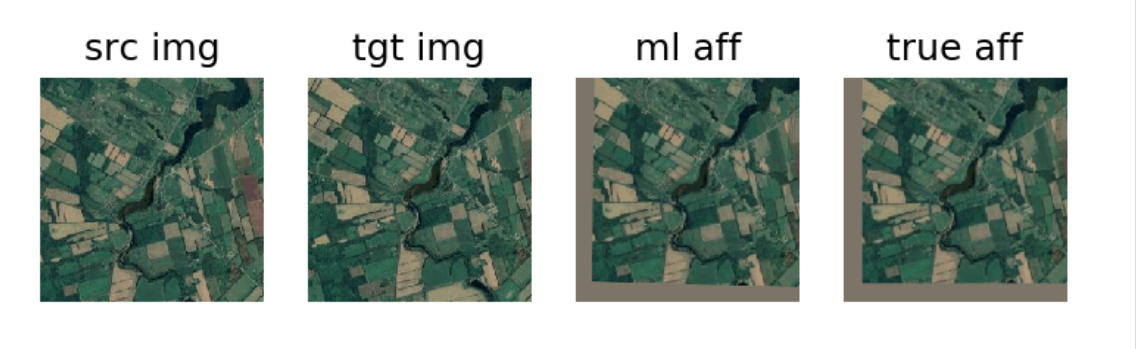
\includegraphics[width = 5.0in]{figs/ml_affine_similar}
\caption{The source (src) and target (tgt) images at left are sent into the machine learning model to produce the affine transformation that may be applied to the source and produce the target. This is shown in the image under heading ml aff. Finally the actual ground truth affine transformation applied to the source image is shown. The ground truth affine transformation represents a shift of 20 pixels to the right and 20 pixels up.}
\end{figure}
  Similar strong results can be seen in Figure 5.2. However even visually in Figure 5.2 we can start to see that the machine learning algorithm contains some errors. Most notably, visually, the image is translated to roughly the correct spot but it has been warped and rotated slightly. The ground truth affine transformation is [[1, 0, 40] [0, 1, 40] [0, 0, 1]]. After normalization this becomes: [[1, 0, -0.3279] [0, 1, -0.3279] [0, 0, 1]] compare to our machine learning algorithm produces an estimated normalized affine transformation of : [[1.0253, -0.0262, -0.2504] [0.0604, 0.9509, -0.2714] [0, 0, 1]],  with a MSE for the normalized affine transformation matrices of 0.0028.\\
\begin{figure}
\centering
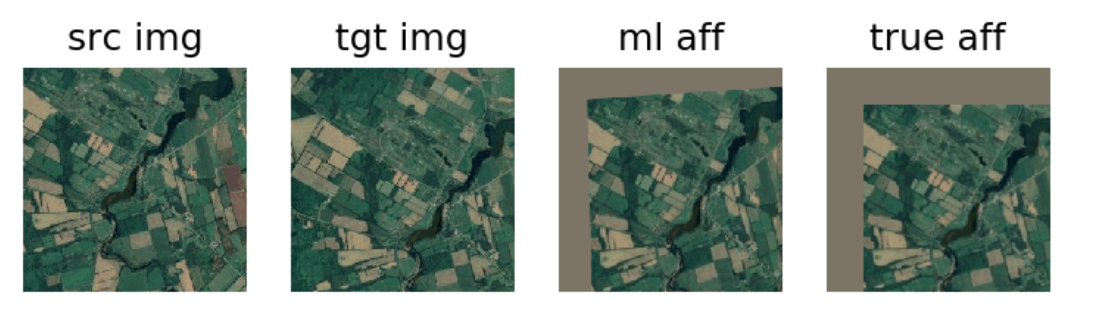
\includegraphics[width = 5.0in]{figs/40_right_40_down}
\caption{Source and Target Images sent into our model produce the ml aff image. Shown last is the actual ground truth solution. The affine transformation for this image pair is a 40 pixel shift right and 40 pixel shift down. Visually our model produces a pleasing result.}
\end{figure}
  In Figure 5.3 we start to see where the model fails. Translations beyond 60 pixels (this figure has a 60 pixel translation to the right and 60 pixels down. The affine transformation for the ground truth and our machine learning estimate are [1, 0, -0.4918] [0, 1, -0.4918] [0, 0, 1]] and [[ 0.8462, -0.0698, -0.0376] [0.0479,  0.8448, -0.0681] [0, 0, 1]] which represents a MSE of 0.0735.
\begin{figure}
\centering
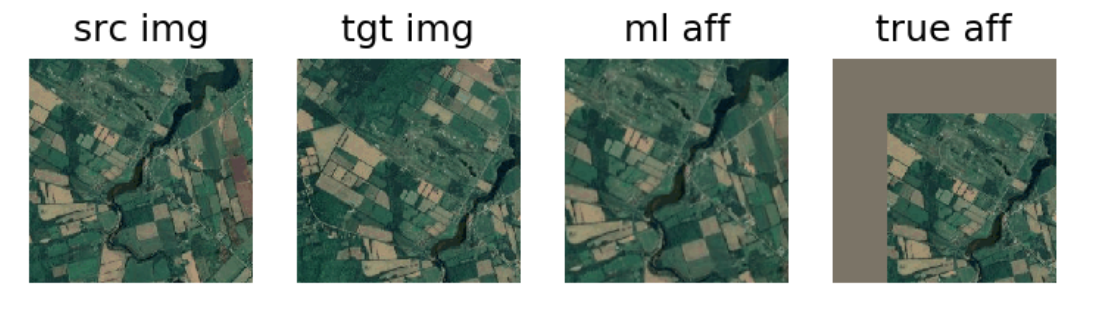
\includegraphics[width = 5.0in]{figs/60_right_60_down}
\caption{Source and Target Images sent into our model produce the ml aff image. Shown last is the actual ground truth solution. The affine transformation for this image pair is a 60 pixel shift right and 60 pixel shift down.}
\end{figure}


\subsection{SIFT and RANSAC}
  The SIFT\cite{lowe2004distinctive} and RANSAC\cite{fischler1981random} algorithms can be uses to find the affine transformation between the source image and the target images. Chapter 2 gives an introductions of SIFT and RANSAC algorithm, we can use SIFT to detect key points in the images, and uses RANSAC to estimate parameters of the transformation.\\
  This section shows a few example images and their affine transformations determined by SIFT and RANSAC. We use the same input images as we used in the machine learning approach, the images are just randomly selected from our dataset representing different degrees of translations.\\
   Figures 5.4, 5.5 and 5.6 show the results when using the SIFT and RANSAC approach. Visually, the method is clearly strong and the alignment is pleasing. The color difference between the unknown portion (black versus grey) left behind after the translation is just an artifact of the display library used to display the images.
   
\begin{figure}
\centering
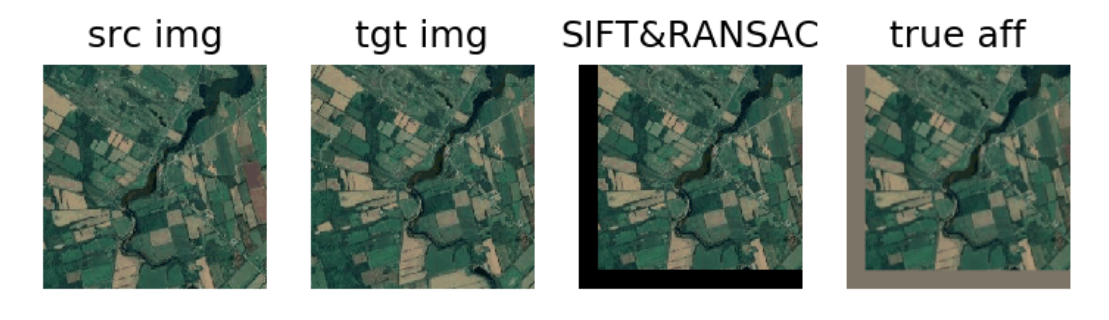
\includegraphics[width = 5.0in]{figs/sift_20r_20up}
\caption{Applying SIFT and RANSAC to the source(src) and target(tgt) images produce the SIFT and RANSAC image are shown. While the ground truth is shown at far right. The ground truth normalized affine transformation matrix is [[1, 0, -0.1639 ] [0, 1, 0.1639] [0, 0, 1]] while with SIFT and RANSAC with normalization we get an affine transformation matrix of [[0.9999, 0.0, -0.1666] [0.0, 0.999, 0.1667] [0, 0, 1]]}
\end{figure}

  
\begin{figure}
\centering
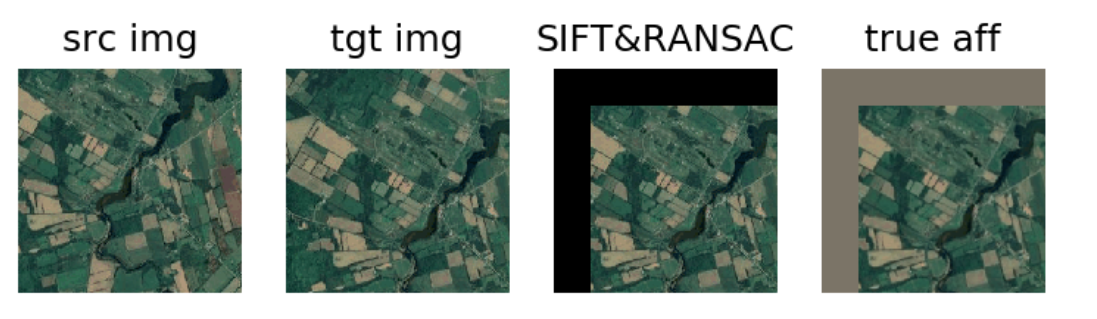
\includegraphics[width = 5.0in]{figs/sift_40down_40right}
\caption{Applying SIFT and RANSAC to the source(src) and target(tgt) images produce the SIFT and RANSAC image are shown. While the ground truth is shown at far right. The ground truth normalized affine transformation matrix is [[1, 0, -0.3279 ] [0, 1, -0.3279] [0, 0, 1]] while with SIFT and RANSAC with normalization we get an affine transformation matrix of [[0.9999, 0.0, -0.3333] [0.0, 0.999, -0.3333] [0, 0, 1]]}
\end{figure}


\begin{figure}
\centering
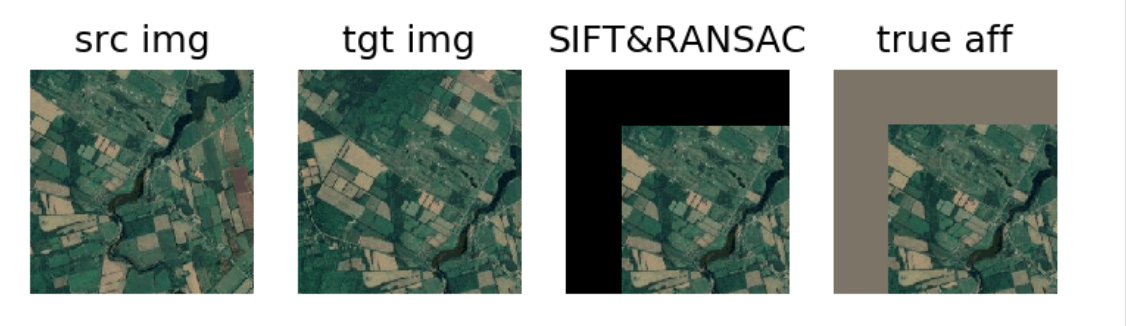
\includegraphics[width = 5.0in]{figs/sift_60down_60right}
\caption{Applying SIFT and RANSAC to the source(src) and target(tgt) images produce the SIFT and RANSAC image are shown. While the ground truth is shown at far right. The ground truth normalized affine transformation matrix is [[1, 0, -0.4918 ] [0, 1, -0.4918] [0, 0, 1]] while with SIFT and RANSAC with normalization we get an affine transformation matrix of [[0.9999, 0.0, -0.4999] [0.0, 0.999, -0.4999] [0, 0, 1]]}
\end{figure}


\subsection{Manual}
We can manually compute an affine transformation matrix by manually identifying the same points in each of the source and target images. We build a small program that produces an affine transformation after we click on three points in the source image and then the same three points in the target image. We do this just by `eyeballing' the same points in each image. The results of this process are shown in Figures 5.7, 5.8 and 5.9.\\
\begin{figure}
\centering
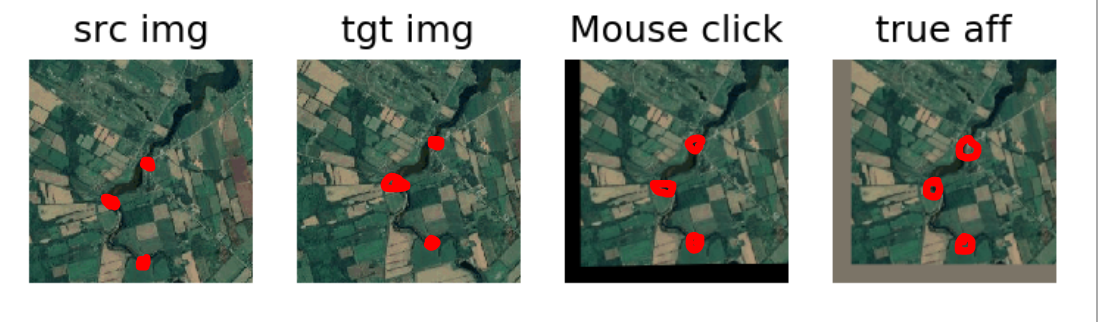
\includegraphics[width = 5.0in]{figs/click_20up_20right}
\caption{We pick 3 points from the source image(src) and 3 point from the target image(tgt) and generated the affine transformation from the points we picked(Mouse click) and compare it with  ground truth affine transformation(true aff).}
\end{figure}
  
 \begin{figure}
\centering
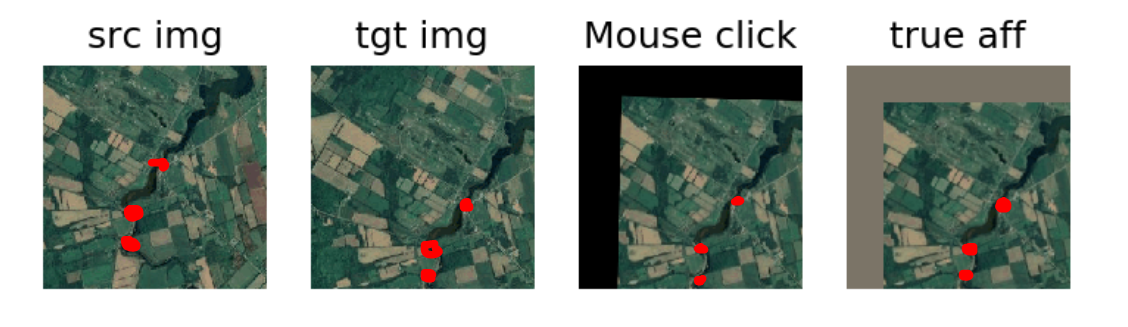
\includegraphics[width = 5.0in]{figs/click_40down_40right}
\caption{We pick 3 points from the source image(src) and 3 point from the target image(tgt) and generated the affine transformation from the points we picked(Mouse click) and compare it with  ground truth affine transformation(true aff).}
\end{figure}

\begin{figure}
\centering
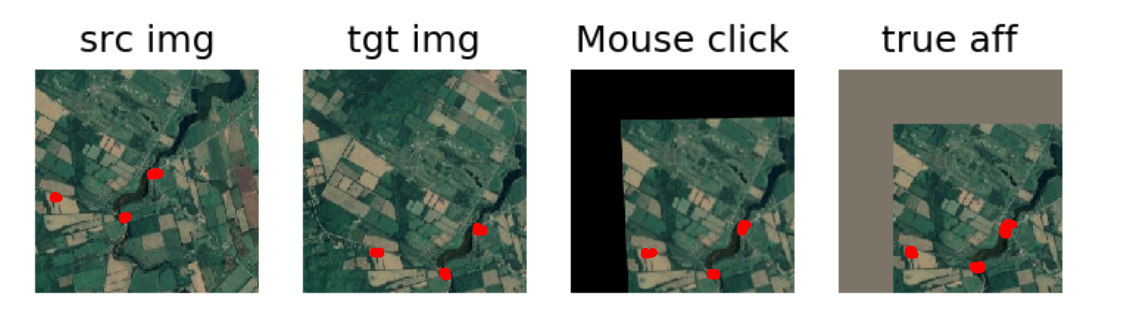
\includegraphics[width = 5.0in]{figs/click_60down_60right}
\caption{We pick 3 points from the source image(src) and 3 point from the target image(tgt) and generated the affine transformation from the points we picked(Mouse click) and compare it with  ground truth affine transformation(true aff).}
\end{figure}

\section{Result}
  We provided the many result examples in the previous section. Visually the model doesn't work well on large translations and the model fails when rotations are involved. In this section we numerically show the accuracy of the model in terms of MSE on our dataset of images. To emphasize the accuracy of the model we break our dataset down into the following subsets, which are chosen based on the degree of translation that they contain.
\begin{itemize}
\item data\_really\_small = A dataset that all the image pairs with translations of 60 or less and rotation.
\begin{itemize}
\item Total loss MSE (1320 images): 20.1473
\item Average loss per image: 0.0153.
\end{itemize}

\item  data\_small\_trans =A dataset that all the image pairs with rotation = 0 and translations of 80 or less.
\begin{itemize}
\item Total loss MSE (1760 images): 79.6672.
\item Average loss per image: 0.0453.
\end{itemize}

\item data\_no\_rot = A dataset that all the image pairs with rotation.
\begin{itemize}
\item Total loss MSE (2640 images):  286.9124.
\item Average loss per image:  0.1087.
\end{itemize}
\end{itemize}
  We can see compare the total loss MSE from these datasets, the data\_really\_small has the smallest error, when the translation is larger, the machine learning approach struggles to find the common features in the image pairsperiod. The model does not estimate large translations (those above 60 pixels) accuractely. In fact we can see in Figure 5.3 an example of this failing. The MSE for this individual example is 0.0735.
 